
\documentclass{tufte-handout}
\usepackage{../../CommonLatexPackages/machine_learning_preamble_1.0}

\fancypagestyle{firstpage}

{\rhead{Module 2 Review \linebreak \textit{Version: \today}}}

\title{Module 2: Review of Main Concepts}
\author{Machine Learning}
\date{Fall 2019}

\invalidatemargin

\begin{document}

\maketitle
\thispagestyle{firstpage}

\begin{learningobjectives}
\bi
\item Review some of the key formulas we've learned.
\item Try some practice problems to firm up the details.
\ei
\end{learningobjectives}

\section{Motivation for the Creation of this Document}

Some folks have expressed that they are having a hard time remembering all of the things they've learned this module.  We are putting together this document to have a single place that lists all of the mathematical and algorithms content we've learned in this module.  We are aiming for a relatively concise resource, so we are avoiding long explanations.  Eventually, we might (or you might via NB?) add pointers to the original assignments that explain this stuff more fully.  An exception to this is that in some cases we have put additional worked examples as appendices to this document (these will be referenced in the text).

\vspace{1em}
\begin{notice}
By creating this document we are not elevating the math / algs portion of this class over the context and ethics or programming parts.  We are creating this resource in response to specific request from a subset of students for more opportunities to reinforce the math / algs for this module.
\end{notice}

\section{Probability}

Probability gives us a formal language to express various forms of uncertainty.  This is hugely valuable when doing machine learning, which often involves many forms of uncertainty (e.g., missing data, model uncertainty, noise in training data, etc.).

\subsection{Probability Space}
Suppose we want to describe some random process in terms of probability.  In order to do so we define a \emph{probability space}.

A probability space consists of two things.
\bi
\item \textbf{Events:} these are things that may or may not occur as a result of our random process.  For example, the event $\mathcal{H}$ might represent the event that when a coin is flipped it comes up heads.
\item \textbf{Probability measure:} this is a function, often called $p$, that assigns a probability to any event.
\ei

In order for $p$ to be a valid probability measure function it must satisfy these three properties.
\be
\item For any event $\mathcal{E}$, $0 \leq p(\mathcal{E}) \leq 1$ (probabilities range from 0, for an impossible event, to 1, for a certain event).
\item For any set of disjoint events, $\mathcal{E}_1, \mathcal{E}_2, \ldots \mathcal{E}_n$ (disjoint events are those that cannot co-occur),
\begin{align}
p(\mathcal{E}_1~\mbox{or}~\mathcal{E}_2 \ldots ~\mbox{or}~\mathcal{E}_n) = \sum_{i=1}^n p(\mathcal{E}_i) \enspace .
\end{align}
\item For any set of exhaustive events, $\mathcal{E}_1, \mathcal{E}_2, \ldots \mathcal{E}_n$, (an exhaustive set of events means at least one \emph{must} occur),
\begin{align}
p(\mathcal{E}_1~\mbox{or}~\mathcal{E}_2 \ldots ~\mbox{or}~\mathcal{E}_n) = 1 \enspace .
\end{align}

\ee

\subsection{Random Variables}
A random variable is a generalization of an event.  Think of a random variable as an entity that takes on a value as a result of a random process.  For instance, one might define a random variable $D$ that captures the rolling a 6-sided die ($D$ would take on a value from the set $\{1, 2, 3, 4, 5, 6\}$.  A random variable consists of two things.
\bi
\item A mapping from each possible outcomes of a random process to a value for the random variable (e.g., our random variable $D$ takes on the value 1 when the roll has comes up 1, value 2 when the roll comes up 2, etc.).
\item A probability mass function (PMF), which provides the probability that a random variable takes on a particular value.  For example, $p(D = 1)$ is the probability that our 6-sided die comes up 1.  Further, if our die is fair, $p(D=1)=\frac{1}{6}$.
\ei

Similar to the conditions for outlined for a probability measure function, a PMF must satisfy the following conditions.
\be
\item If $V$ is the set of all possible values that the random variable $X$ can take on, then $0 \leq p(X = x) \leq 1$ for any value $x$ in the set $V$.
\item If we add the probability of all possible values that $X$ can take on, we should get $1$.  That is, $\sum_{x \in V} p(X = x) = 1$.
\ee

\begin{notice}
In pretty much all of the content in this module any rule that works for events will also work for random variables.  For instance, Bayes' rule for events $\mathcal{A}$ and $\mathcal{B}$ is $p(\mathcal{A} | \mathcal{B}) = \frac{p(\mathcal{B}|\mathcal{A}) p(\mathcal{A})}{p(\mathcal{B})}$.  This equation looks the same as Bayes' rule for two random variables $X$ and $Y$, $p(X=x | Y=y) = \frac{p(Y=y|X=x) p(X=x)}{p(Y=y)}$.  As a result, when we present a rule for manipulating the probability of various events, you can also assume that it will work with little modification for random variables.  In order to make this document simpler, we won't explicitly give the analogous formula for random variables, but if you have any questions on what it would look like, please post on NB.
\end{notice}

\subsection{Complement Rule}

If we know the probability of an event $\mathcal{E}$ occurring, then the probability of it not occurring $p(\neg \mathcal{E})$ is given by the formula

\begin{align}
p(\neg \mathcal{E}) = 1 - p(\mathcal{E}) \enspace .
\end{align}

\subsection{Conditional Probability}
A conditional probability tells us the probability of some event occurring assuming (or conditioned on) another event having occurred.  For instance, we could say ``what is the probability that we observe a particular symptom given that a person has a disease?''  Conditional probability is defined using the following equation.

\begin{align}
p(\mathcal{A}|\mathcal{B}) &= \frac{p(\mathcal{A}, \mathcal{B})}{p(\mathcal{B})}
\end{align}

The term $p(\mathcal{A}, \mathcal{B})$ is known as a joint probability, which we will define in the next section.

\subsection{Joint Probability}
The probability of two events, $\mathcal{A}$ and $\mathcal{B}$, both occurring is called the joint probability of $\mathcal{A}$ and $\mathcal{B}$.  We write this as:
\begin{align}
p(\mathcal{A}, \mathcal{B}) &= \mbox{the probability of both $\mathcal{A}$ and $\mathcal{B}$ simultaneously occurring}
\end{align}

For any two events $\mathcal{A}$ and $\mathcal{B}$, we can write the joint probability in terms of the product of a marginal probability (the probability of one of the events) and a conditional probability.
\begin{align}
p(\mathcal{A}, \mathcal{B}) &= p(\mathcal{A}) p( \mathcal{B} | \mathcal{A})  \\
&= p(\mathcal{B}) p( \mathcal{A} | \mathcal{B})
\end{align}


\subsection{Marginalization}
If we can easily compute the joint distribution of two events (that is $p(\mathcal{A}, \mathcal{B})$), then we can use the technique of marginalization to obtain the \emph{marginal distribution} (the probability of just one of the events in isolation).

\begin{align}
p(\mathcal{A}) &= p(\mathcal{A}, \mathcal{B}) + p(\mathcal{A}, \neg \mathcal{B})
\end{align}

It's worth giving the translation of this to random variables explicitly.  If $X$ and $Y$ are random variables and $V$ contains all possible values that $X$ can take on, then
\begin{align}
p(Y=y) &= \sum_{x \in V} p(Y=y, X=x) \enspace .
\end{align}

TODO: we can also think of marginalization using tree.

\subsection{Product Rule}

We can decompose the joint probability of a bunch of events into a product of probabilities.  Suppose $\mathcal{E}_1, \mathcal{E}_2, \ldots, \mathcal{E}_n$ represent events, then
\begin{align}
p(\mathcal{E}_1, \mathcal{E}_2, \ldots, \mathcal{E}_n) &= p(\mathcal{E}_1) p(\mathcal{E}_2 | \mathcal{E}_1) p(\mathcal{E}_3 | \mathcal{E}_1, \mathcal{E}_2) \ldots p(\mathcal{E}_n | \mathcal{E}_1, \ldots, \mathcal{E}_{n-1}) \enspace .
\end{align}
The rule we're applying here is to start with an event conditioned on nothing, then multiply by the next event conditioned on the previous event, then multiply by the next event conditioned on the previous two, etc.  The order in which you select the events is also arbitrary, so if $n=3$, the following are equivalent.
\begin{align}
p(\mathcal{E}_1, \mathcal{E}_2, \mathcal{E}_3) &= p(\mathcal{E}_1) p(\mathcal{E}_2|\mathcal{E}_1)p(\mathcal{E}_3|\mathcal{E}_1, \mathcal{E}_2) \nonumber \\
&= p(\mathcal{E}_2) p(\mathcal{E}_3|\mathcal{E}_2)p(\mathcal{E}_1|\mathcal{E}_2, \mathcal{E}_3) \nonumber \\
&= p(\mathcal{E}_3) p(\mathcal{E}_2|\mathcal{E}_3)p(\mathcal{E}_1|\mathcal{E}_3, \mathcal{E}_2) \nonumber \\
&\mbox{... there are three more potential orderings that we won't give explicitly} \nonumber
\end{align}

\subsection{Bayes' Rule}

Bayes' rule lets you take a conditional probability $p(\mathcal{A}|\mathcal{B})$ and flip the order of the events across the conditioning bar.
\begin{align}
p(\mathcal{A}|\mathcal{B}) &= \frac{p(\mathcal{B}|\mathcal{A}) p(\mathcal{A})}{p(\mathcal{B})}
\end{align}

There are a few alternate forms of Bayes' rule.
\bi
\item You can move multiple events through the conditioning bar (here are two examples where we move two events, but you can move any number of events).
\begin{align}
p(\mathcal{A}, \mathcal{B} | \mathcal{C}) &= \frac{p(\mathcal{C}|\mathcal{A}, \mathcal{B}) p(\mathcal{A}, \mathcal{B})}{p(\mathcal{C})} \\
p(\mathcal{A} |  \mathcal{B}, \mathcal{C}) &= \frac{p(\mathcal{B}, \mathcal{C}|\mathcal{A}) p(\mathcal{A})}{p(\mathcal{B}, \mathcal{C})}
\end{align}
\item You don't have to swap all of the events across the conditioning bar (e.g., below, we leave $\mathcal{C}$ on the righthand side of the bar).
\begin{align}
p(\mathcal{A}|\mathcal{B},\mathcal{C}) &= \frac{p(\mathcal{B} | \mathcal{A}, \mathcal{C}) p(\mathcal{A}|\mathcal{C})}{p(\mathcal{B}|\mathcal{C})}
\end{align}
\ei


\paragraph{What's the big deal about Bayes?}
Here are two potential answers to this.
\bi
\item It helps us compute probabilities of interest.  Sometimes it is much more natural to compute $p(\mathcal{B} | \mathcal{A})$, then $p(\mathcal{A} | \mathcal{B})$.  For example, if $\mathcal{A}$ represents the event that someone has a particular disease and $\mathcal{B}$ represents someone exhibiting a particular symptom, since we think of the disease as causing the symptom it may be easier to model the probability of the symptom given the disease.  It is less natural to think of the probability of the disease given the symptom since we don't typically think of a symptom as causing a disease.
\item Consider watching Julia Galef's \href{https://www.youtube.com/watch?v=za7RqnT7CM0}{Bayes: How one equation changed the way I think}
\ei


\subsection{Independence}

Two events $\mathcal{A}$ and $\mathcal{B}$ are independent (written as $\mathcal{A} \condindep \mathcal{B}$) if and only if
\begin{align}
p(\mathcal{A}, \mathcal{B}) = p(\mathcal{A}) p(\mathcal{B}) \enspace .
\end{align}
This equation also implies the following very useful rule.
\begin{align}
p(\mathcal{A} | \mathcal{B}) = p(\mathcal{A}) \enspace .
\end{align}
Intuitively, we can drop $\mathcal{B}$ from the right side of the conditioning bar since knowing that $\mathcal{B}$ occurred doesn't change the probability of $\mathcal{A}$.


\subsection{Conditional Independence}


Two events $\mathcal{A}$ and $\mathcal{B}$ are conditionally independent given a third event $\mathcal{C}$ (written as $\mathcal{A} \condindep \mathcal{B}~|~\mathcal{C}$) if and only if
\begin{align}
p(\mathcal{A}, \mathcal{B} | \mathcal{C}) = p(\mathcal{A} | \mathcal{C}) p(\mathcal{B} | \mathcal{C}) \enspace .
\end{align}
This equation also implies the following very useful rule.
\begin{align}
p(\mathcal{A} | \mathcal{B}, \mathcal{C}) = p(\mathcal{A} | \mathcal{C}) \enspace .
\end{align}
The intuition is that we can drop $\mathcal{B}$ from the right side of the conditioning bar since knowing that $\mathcal{B}$ occurred doesn't change the probability of $\mathcal{A}$ if we already know that $\mathcal{C}$ occurred.


\section{Bayesian Networks}

A Bayesian Network (BN) defines a model consisting of one or more events or random variables.  A BN consists of the following components.
\bi
\item A graph, that encodes the dependencies between the random variables and events.  This graph contains nodes and directed edges.  We can think of an edge that goes from node $A$ to node $B$ as indicating that $A$ causes $B$.
\item A conditional probability table that indicates the probability that a node takes on a particular value given the values of its parents.  Note: that on the next assignment when we generalize these networks to contain continuous values, these probability tables will be modified.
\ei

Here is an example of a BN that represents how two people, Mary and John, respond to an alarm in their apartment complex.  The alarm is triggered by earthquakes and burglaries.

\begin{center}
\includegraphics[width=0.6\linewidth]{../02/figures/maryjohn}
\end{center}

The circles in this graph (called nodes) are the various events.  Each of these can either be true or false (as stated before, nodes can also represent random variables that can take on multiple values).  The arrows indicate causal relationships (e.g., the alarm going off is caused by burglaries and earthquakes).  The tables next to each node give us the probability of the node conditioned on its parents.

 The condition that must hold for any BN is that if we write the joint distribution of all of the random variables (or events, the relationship is the same for either) in the network, it must factorize in the following way (we'll use $X_1, X_2, \ldots X_n$ to represent random variables in the network and we'll define the function $Pa(X_i)$ to return all of the random variables that are parents of $X_i$).

\begin{align}
p(X_1, X_2, \ldots, X_n) &= p(X_1 | Pa(X_1)) p(X_2 | Pa(X_2)) \ldots p(X_n | Pa(X_n)) \label{eq:bnparents}
\end{align}

\begin{exercise}
For practice, use Equation~\ref{eq:bnparents} to factor $p(\mathcal{B}, \mathcal{E}, \mathcal{A}, \mathcal{J}, \mathcal{M})$ for the alarm network.
\end{exercise}

\subsection{D-Separation}
One of the beautiful things at BNs is that they allow us to infer independence relationships from the graph structure.  In assignment 2 we gave some resources to learn about d-separation.  We encourage you to take a second look at those if you are having trouble (one was a video and one was a document).  If you find any other good resources on d-separation, please share them here.  Next, we'll try to state the rules of d-separation as clearly and concisely as possible.

\begin{recall}[Definition of D-Separation]
Two nodes, $\mathcal{A}$ and $\mathcal{B}$, in a BN are d-separated when conditioning on a set of nodes, $\mathcal{C}$, if and only if \emph{all} paths between  $\mathcal{A}$ and $\mathcal{B}$ are blocked when conditioning on $\mathcal{C}$ (the concept of \emph{blocked} will be defined below).  Note that a path consists of traversing one or more edges, in sequence, of a BN (irrespective of the direction of the edge).  A path between $\mathcal{A}$ and $\mathcal{B}$ conditioned on nodes $\mathcal{C}$ if any of the following conditions are met.
\be
\item The path contains a collider and neither the collider nor any of its descendants are in the set $\mathcal{C}$ (a collider is a node where the path consists of two incoming arrows, e.g., $\mathcal{D} \rightarrow \mathcal{E} \leftarrow \mathcal{F}$).
\item The path contains a segment that looks like $\mathcal{D} \rightarrow \mathcal{E} \rightarrow \mathcal{F}$ and $\mathcal{E}$ is in the set $\mathcal{C}$ (i.e., we are conditioning on $\mathcal{E}$).
\item The path contains a segment that looks like $\mathcal{D} \leftarrow \mathcal{E} \rightarrow \mathcal{F}$ and $\mathcal{E}$ is in the set $\mathcal{C}$ (i.e., we are conditioning on $\mathcal{E}$).
\ee


\vspace{1em}
\noindent If $\mathcal{A}$ and $\mathcal{B}$ are d-separated conditioned on $\mathcal{C}$, then $\mathcal{A} \condindep \mathcal{B}~|~\mathcal{C}$.

\end{recall}

\begin{exercise}
Choose two nodes in the alarm network.  Are they independent?  How would this change if you conditioned on each of the other three nodes in the network?  Repeat this exercise for other pairs of nodes in the network.
\end{exercise}

\section{Fairness Criteria for ML}

TODO

\section{Na\"ive Bayes}

The Na\"ive Bayes model can be described using the following BN.

\begin{center}
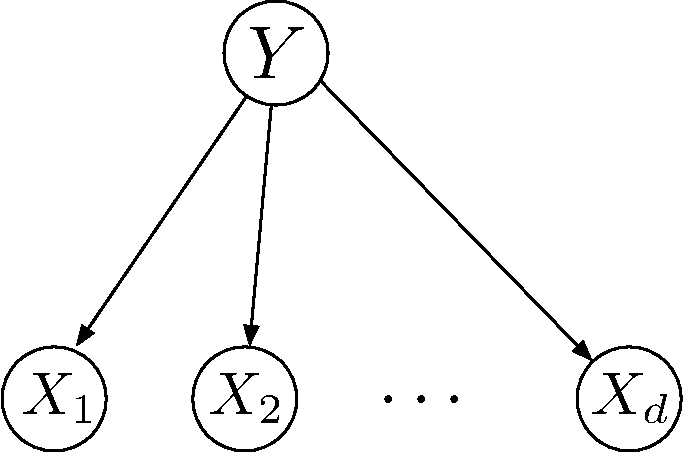
\includegraphics[width=0.3\linewidth]{../02/figures/naivebayesgm}
\end{center}

Remember, that in order to define the BN we need to also specify the conditional probability tables (the probability of each node conditioned on its parents).  For the Na\"ive Bayes model this consists of the following probabilities.

\bi
\item If $Y$ is a random variable, you need $p(Y=i)$ (for all possible values, $i$, that $Y$ could take on).  If $\mathcal{Y}$ is an event, you would need $p(\mathcal{Y})$.
\item If the $X_i$'s are random variables, you need $p(X_i=j | Y=k)$ (for all values, $k$, that $Y$ can take on and all possible values, $j$, that the $X_i$ can take on).
\ei

As a motivating example, let's look back at the Titanic dataset from the last module.  A potential BN for the Titanic dataset is shown below.

\begin{center}
\includegraphics[width=0.8\linewidth]{../02/figures/titanicbn}
\end{center}

You'll notice that one of the nodes in this graph is a random variables (\emph{fare class}) and some are events (\emph{survived}, \emph{male}, and \emph{young}).  The conditional probabilities were determined using the technique of maximum likelihood estimation (MLE) (which we will describe later).  In this case, MLE simply consists of counting the number of times one of the nodes takes on a particular value when the parent also takes a particular value and normalizing over all possible values the node can take on (more on this in the next section).

\section{Maximum Likelihood Estimation}


\section{N-Grams and Sequence Analysis}


\section{Are we missing anything?}
Keep in mind that this document's scope is within the math / algorithms part of this class (not on the context and ethics or programming side).  Comment on NB here to request stuff to add. 

\end{document}
